\documentclass{article}

% if you need to pass options to natbib, use, e.g.:
%     \PassOptionsToPackage{numbers, compress}{natbib}
% before loading neurips_2020

% ready for submission
% \usepackage{neurips_2020}

% to compile a preprint version, e.g., for submission to arXiv, add add the
% [preprint] option:
%     \usepackage[preprint]{neurips_2020}

% to compile a camera-ready version, add the [final] option, e.g.:
     \usepackage[final]{neurips_2020}

% to avoid loading the natbib package, add option nonatbib:
    % \usepackage[nonatbib]{neurips_2020}

\usepackage[utf8]{inputenc} % allow utf-8 input
\usepackage[T1]{fontenc}    % use 8-bit T1 fonts
\usepackage{hyperref}       % hyperlinks
\usepackage{url}            % simple URL typesetting
\usepackage{booktabs}       % professional-quality tables
\usepackage{amsfonts}       % blackboard math symbols
\usepackage{nicefrac}       % compact symbols for 1/2, etc.
\usepackage{microtype}      % microtypography
\usepackage{amsmath,amsthm,amssymb,setspace, mathtools, enumitem}
\usepackage{color}   %May be necessary if you want to color links
\usepackage{hyperref}
\hypersetup{
	colorlinks=true, %set true if you want colored links
	linktoc=all,     %set to all if you want both sections and subsections linked
	linkcolor=black,  %choose some color if you want links to stand out
	urlcolor=cyan
}

\title{Final Report \\ STAT 689 Spring 2022 }

% The \author macro works with any number of authors. There are two commands
% used to separate the names and addresses of multiple authors: \And and \AND.
%
% Using \And between authors leaves it to LaTeX to determine where to break the
% lines. Using \AND forces a line break at that point. So, if LaTeX puts 3 of 4
% authors names on the first line, and the last on the second line, try using
% \AND instead of \And before the third author name.

\author{%
  Carson James\\
  Department of Statistics\\
  Texas A\&M University\\
  College Station, TX 77840 \\
  \texttt{carsonaj@tamu.edu} \\
  % examples of more authors
  % \And
  % Coauthor \\
  % Affiliation \\
  % Address \\
  % \texttt{email} \\
  % \AND
  % Coauthor \\
  % Affiliation \\
  % Address \\
  % \texttt{email} \\
  % \And
  % Coauthor \\
  % Affiliation \\
  % Address \\
  % \texttt{email} \\
  % \And
  % Coauthor \\
  % Affiliation \\
  % Address \\
  % \texttt{email} \\
}


\theoremstyle{definition}
\newtheorem{definition}{Definition}[subsection]
\newtheorem{defn}[definition]{Definition}
\newtheorem{note}[definition]{Note}
\newtheorem{thm}[definition]{Theorem}
\newtheorem{lem}[definition]{Lemma}
\newtheorem{prop}[definition]{Proposition}
\newtheorem{cor}[definition]{Corollary}
\newtheorem{conj}[definition]{Conjecture}
\newtheorem{ex}[definition]{Exercise}
\newtheorem{apprx}[definition]{Approximation}
\newtheorem{modl}[definition]{Model}


\newcommand{\al}{\alpha}
\newcommand{\gam}{\gamma}
\newcommand{\Gam}{\Gamma}
\newcommand{\be}{\beta} 
\newcommand{\del}{\delta} 
\newcommand{\Del}{\Delta}
\newcommand{\lam}{\lambda}  
\newcommand{\Lam}{\Lambda} 
\newcommand{\ep}{\epsilon}
\newcommand{\sig}{\sigma} 
\newcommand{\om}{\omega}
\newcommand{\Om}{\Omega}
\newcommand{\C}{\mathbb{C}}
\newcommand{\N}{\mathbb{N}}
\newcommand{\E}{\mathbb{E}}
\newcommand{\Z}{\mathbb{Z}}
\newcommand{\R}{\mathbb{R}}
\newcommand{\T}{\mathbb{T}}
\newcommand{\Q}{\mathbb{Q}}
\renewcommand{\P}{\mathbb{P}}
\newcommand{\MA}{\mathcal{A}}
\newcommand{\MC}{\mathcal{C}}
\newcommand{\MB}{\mathcal{B}}
\newcommand{\MF}{\mathcal{F}}
\newcommand{\MG}{\mathcal{G}}
\newcommand{\ML}{\mathcal{L}}
\newcommand{\MN}{\mathcal{N}}
\newcommand{\MS}{\mathcal{S}}
\newcommand{\MP}{\mathcal{P}}
\newcommand{\ME}{\mathcal{E}}
\newcommand{\MT}{\mathcal{T}}
\newcommand{\MM}{\mathcal{M}}
\newcommand{\MI}{\mathcal{I}}
\newcommand{\MU}{\mathcal{U}}
\newcommand{\MO}{\mathcal{O}}

\newcommand{\ui}{[0,1]}
\newcommand{\p}{\partial}

\newcommand{\io}{\text{ i.o.}}
%\newcommand{\ev}{\text{ ev.}}
\renewcommand{\r}{\rangle}
\renewcommand{\l}{\langle}

\newcommand{\RG}{[0,\infty]}
\newcommand{\Rg}{[0,\infty)}
\newcommand{\Ru}{(\infty, \infty]}
\newcommand{\Rd}{[\infty, \infty)}
\newcommand{\Ll}{L^1_{\text{loc}}(\R^n)}

\newcommand{\limfn}{\liminf \limits_{n \rightarrow \infty}}
\newcommand{\limpn}{\limsup \limits_{n \rightarrow \infty}}
\newcommand{\limn}{\lim \limits_{n \rightarrow \infty}}
\newcommand{\convt}[1]{\xrightarrow{\text{#1}}}
\newcommand{\conv}[1]{\xrightarrow{#1}} 
\newcommand{\seq}[2]{(#1_{#2})_{#2 \in \N}}

\newcommand{\lsc}{l.s.c. }

\newcommand{\as}[1]{\overset{#1}{\sim}}
\newcommand{\astx}[1]{\overset{\text{#1}}{\sim}}

\DeclareMathOperator{\supp}{supp}
\DeclareMathOperator{\sgn}{sgn}
\DeclareMathOperator{\spn}{span}
\DeclareMathOperator{\iso}{Iso}
\DeclareMathOperator{\id}{id}
\DeclareMathOperator{\argmax}{arg\,max}
\DeclareMathOperator{\argmin}{arg\,min}
\DeclareMathOperator{\Aut}{Aut}
\DeclareMathOperator{\Homeo}{Homeo}
\DeclareMathOperator{\Sym}{Sym}
\DeclareMathOperator{\cl}{cl}
\DeclareMathOperator{\intt}{int}


\begin{document}

\maketitle

\begin{abstract}
  This report will discuss an approximation to the posterior mean of a Gaussian process by a neual network that improves over the computational efficiency and true data generating function estimation accuracy of the exact posterior mean. 
\end{abstract}

\section{Background}
\begin{note}
The approximation relies upon tools from the theory of Gaussian processes, Banach spaces, Hilbert spaces, reproducing kernel Hilbert spaces and convex analysis. The relevant results will be mentioned. 
\end{note}

\begin{defn}
Let $T$ be a set and $c: T^2 \rightarrow \R$. Then $c$ is said to be \textbf{positive definite} if for each $(x_j)_{j=1}^n \in T^n$, the matrix $c(x,x)$ is positive definite. 
\end{defn}

\begin{defn}
Let $T$ be a set, $(\Om, \MF, P)$ a probability space, $\mu : T \rightarrow \R$, $c: T^2 \rightarrow \R$ symmetric and positive definite and $f: T \rightarrow L^2(\Om, \MF, P)$ (i.e. $f$ is a random function from $T$ to $\R$). Then $f$ is said to be a \textbf{Gaussian Process} with mean function $\mu$ and covariance function $c$, denoted $f \sim GP(\mu, c)$, if for each $x = (x_j)_{j=1}^n \in T^n$, $f(x) \sim N_{n}(\mu(x), c(x,x))$. 
\end{defn}

\begin{thm}
Let $T$ be a set, $c: T^2 \rightarrow \R$ positive definite, $x = (x_j)_{j=1}^n \in T^n$, $y = (y_j)_{j=1}^n \in \R^n$. Suppose we have the following model:
\begin{align*}
y_i &= f(x_i) + \ep_i \\
\ep_i &\sim N(0, \sig^2) \\
f &\sim GP(0, c)
\end{align*}
Then $$f|x, y \sim GP(\tilde{\mu}, \tilde{c})$$ where $$\tilde{\mu}(t) = c(t, x)[c(x,x) + \sig^2I]^{-1}y$$ and $$\tilde{c}(s,t) = c(s,t) - c(s,x)[c(x,x) + \sig^2 I]^{-1}c(x,t)$$

\end{thm}

\begin{defn} \textbf{Frechet Derivative:} \\
	Let $X, Y$ be a banach spaces, $A \subset X$ open, $f:A \rightarrow Y$ and $x_0 \in A$. 
	\begin{itemize}
	\item Then $f$ is said to be \textbf{ Frechet differentiable at $x_0$} if there exists $Df(x_0) \in L(X,Y)$ such that, $$f(x_0 + h) = f(x_0) + Df(x_0)(h) + o(\|h\| ) \hspace{.5cm} \text{ as } h \rightarrow 0$$  
	\item If $f$ is Frechet differentiable at $x_0$, we define the \textbf{ Frechet derivative of $f$ at $x_0$} to be $Df(x_0)$. 
	\item We say that $f$ is \textbf{ Frechet differentiable} if for each $x \in A$, $f$ is Frechet differentiable at $x$. 
	\item If $f$ is Frechet differentiable, we define the \textbf{ Frechet derivative of $f$}, denoted $Df:A \rightarrow L(X, Y)$, by $x \mapsto D^{(1)}f(x)$. 
	\end{itemize}
	\end{defn}
	
	\begin{thm}
	Let $X$ be a Banach space, $f:X \rightarrow \R$ and $x_0 \in X$. If $f$ is Frechet differentiable at $x_0$ and $f$ has a local minimum at $x_0$, then $Df(x_0) = 0$. 
	\end{thm}
	
	\begin{thm}
Let $X$ be a Banach space and $f:X \rightarrow \R$ be continuously second order Frechet differentiable. If for each $x \in X$, $D^2f(x)$ is positive definite, then $f$ is strictly convex.
\end{thm}

\begin{defn} 
	Let $H$ be a Hilbert space, $f: H \rightarrow \R$ and $x_0 \in H$. Suppose that $f$ is Frechet differentiable at $x_0$. Then $Df(x_0) \in H^*$. We define the \textbf{gradient of $f$ at $x_0$}, denoted $\nabla f(x_0) \in H$, via the Riesz representation theorem to be the unique element of $H$ satisfying $$\l \nabla f(x_0), y \r = Df(x_0)(y) \hspace{.3cm} \text{ for each } y \in H$$
	\end{defn}


\begin{defn}
Let $T$ be a set and $H \subset \R^T$ a hilbert space. For $t \in T$, we define the \textbf{evaluation functional at $t$}, denoted $l_t : H \rightarrow \R$, by $$l_t(f) = f(t)$$ 
The space $H$ is said to be a \textbf{reproducing kernel Hilbert space (RKHS)} if for each $t \in T$, $l_t \in H^*$ (i.e. $l_t$ is bounded). \\
If $H$ is an RKHS, the Riesz representation theorem implies that for each $t \in T$, there exists $c_t \in H$ such that for each $f \in H$, $\l c_t, f\r = f(t)$. \\

If $H$ is an RKHS, we define the \textbf{reproducing kernel} associated to $H$, denoted $c_H:T^2 \rightarrow \R$, by $$c_H(s,t) = \l c_s, c_t \r$$ 
\end{defn}
	
\begin{thm}
Let $T$ be a set and $c : T^2 \rightarrow \R$. If $c$ is symmetric and positive definite, then there exists a unique reproducing kernel Hilbert space $H \subset \R^T$ such that $c_H = c$.
\end{thm}

\begin{defn}
Let $T$ be a set, $c : T^2 \rightarrow \R$ a symmetric, postivie definite kernel on $T$, $H \subset \R^T$ the corresponding RKHS, $x = (x_j)_{j=1}^n \in T^n$, $\lam > 0$ and $y = (y_j)_{j=1}^n \in \R^n$. \\
Define $L_{\lam, y}: H \rightarrow \R$ by $$L_{\lam, y}(f) = \sum_{j=1}^n (y_j - f(x_j) )^2 + \lam \|f\|_H^2$$ \\
and set $$\hat{f}_{\lam, y} = \argmin\limits_{f \in H}L_{\lam, y}(f)$$ 
\\
\end{defn}

\begin{thm}
Let $T$ be a set, $c : T^2 \rightarrow \R$ a symmetric, postivie definite kernel on $T$, $H \subset \R^T$ the corresponding RKHS, $x = (x_j)_{j=1}^n \in T^n$, $\lam > 0$ and $y = (y_j)_{j=1}^n \in \R^n$. \\
Then $L_{\lam, y}$ is strictly convex.
\end{thm}

\begin{thm}
Let $T$ be a set, $c : T^2 \rightarrow \R$ a symmetric, postivie definite kernel on $T$, $H \subset \R^T$ the corresponding RKHS, $x = (x_j)_{j=1}^n \in T^n$, $\lam > 0$ and $y = (y_j)_{j=1}^n \in \R^n$. \\
Then there exist $(\hat{\al}_j)_{j=1}^n \subset \R$ such that $$\hat{f}_{\lam, y}(t) = \sum_{j=1}^n \hat{\al}_jc(t, x_j)$$
Standard multivariable calculus shows that $\hat{\al} = (c(x,x) + \lam I)^{-1}y$ so that 
$$\hat{f}_{\lam, y}(t) = c(t,x)(c(x,x) + \lam I)^{-1}y$$
\end{thm}

\begin{note}
The above results tell us that in the context of Gaussian processes, 
$$\hat{f}_{\sig^2, y} = \tilde{\mu}$$
\end{note}

\section{Approximation}

\begin{lem}
Let $T$ be a set, $c : T^2 \rightarrow \R$ a symmetric, postivie definite kernel on $T$, $H \subset \R^T$ the corresponding RKHS, $x = (x_j)_{j=1}^n \in T^n$, $\lam > 0$ and $y = (y_j)_{j=1}^n \in \R^n$. \\
Then for each $f_0 \in H$, 
$$\nabla L_{\lam, y}(f_0) = 2\bigg [ \sum_{j=1}^n (f_0(x_j)- y_j) c_{x_j} + \lam f_0\bigg ]$$
\end{lem}


\begin{apprx}
The preceeding lemma implies that in the context of Gaussian processes, we have that 
\begin{align*}
\nabla L_{\lam, y}(\tilde{\mu}) 
&= 2\bigg [ \sum_{j=1}^n (\tilde{\mu}(x_j)- y_j) c_{x_j} + \sig^2 \tilde{\mu} \bigg ] \\
&= 0
\end{align*}

Thus, if we approximate $\tilde{\mu}$ by a neural network $g_{\theta}:T \rightarrow \R$, we obtain the restriction that for each $t \in T$, 
$$\sum_{j=1}^n (g_{\theta}(x_j)- y_j) c_{x_j}(t) + \sig^2 g_{\theta}(t) = 0$$ 
So we may make a grid $(t_k)_{k=1}^a \subset T$ and for each $k \in \{1, \ldots, a\}$, 
 $$\sum_{j=1}^n (g_{\theta}(x_j)- y_j) c_{x_j}(t_k) + \sig^2 g_{\theta}(t_k) = 0$$ 
 Now, taking absolute values or squares and summing we obtain the following restrictions: 
 \begin{itemize}
 \item $$\sum_{k=1}^a \bigg |\sum_{j=1}^n (g_{\theta}(x_j)- y_j) c_{x_j}(t_k) + \sig^2 g_{\theta}(t_k) \bigg| = 0$$ 
 \item $$\sum_{k=1}^a \bigg (\sum_{j=1}^n (g_{\theta}(x_j)- y_j) c_{x_j}(t_k) + \sig^2 g_{\theta}(t_k) \bigg)^2 = 0$$
\end{itemize}  
Finally, using the triangle inequality and Jensen's inequality we obtain the following loss functions:
\begin{itemize}
\item $$l_1(\theta) = \sum_{k=1}^a \bigg[ \sum_{j=1}^n |(g_{\theta}(x_j)- y_j)| c_{x_j}(t_k) + \sig^2 |g_{\theta}(t_k)| \bigg] $$ 
\item $$l_2(\theta) = \sum\limits_{k=1}^a \bigg[ \bigg (\sum\limits_{j=1}^n (g_{\theta}(x_j) - y_j)c_{x_j}(t_k)\bigg)^2 + \sig^4 g_{\theta}(t_k)^2\bigg]$$\\
\end{itemize}
\end{apprx}

\begin{note}
Either loss function $l_1$ or $l_2$ lets us train $g_{\theta}$ to approximate the exact posterior mean $\tilde{\mu}$. However in many cases the exact posterior mean does not align with a true data generating function $f_0$ (if there is one) in our regression model. We address this in the following approximation model.
\end{note}
\newpage

\begin{apprx}
To augment the loss function $l \in \{l_1, l_2\}$, we add an additional MSE term: 
$$MSE(\theta) = \sum_{j=1}^n (g_{\theta}(x_j) - y_j)^2$$ For $\al \in (0,1)$, we weight the original loss functions and the MSE term in order to obtain the following augmented loss functions:
\begin{itemize}
\item $l'_1(\theta) = \al l_1(\theta) + (1-\al) \text{MSE}(\theta)$\\
\item $l'_2(\theta) = \al l_2(\theta) + (1-\al) \text{MSE}(\theta)$\\
\end{itemize}
\end{apprx}

\begin{note}
The motivation for the augmented loss function is to choose $\al > 0.5$ so that we have an overall behavior similar to that of the exact posterior mean, but within the data, the MSE term dominates and we have a better fit to the true data generating function. 
\end{note}



\section{Results}

\begin{modl}
We generated data according to the following model:
\begin{align*}
y_i &= f_0(x_i) + \ep_i \\
\ep_i &\sim N(0, 0.1^2) \\
x_i & \sim \text{U(0,4)} \\
f_0(x) &= 2e^{-x} +  0.5 \cos(8x) + 4
\end{align*}
and trained a neural network $g_{\theta}$ on the grid of evenly spaced grid $(t_k)_{k=1}^{40} \subset [0,40]$.
\end{modl}

\begin{note}
Below we show the results after training $g_{\theta}$ with the $l_2$ loss function (RKHS NN), the $l'_2$ loss function with $\al = 0.7$ (RKHS-MSE mix NN) and the MSE loss function (MSE NN). We included photos to compare performance inside the data on $[0,4]$ and outside the data on $[0, 15]$. 
\end{note}


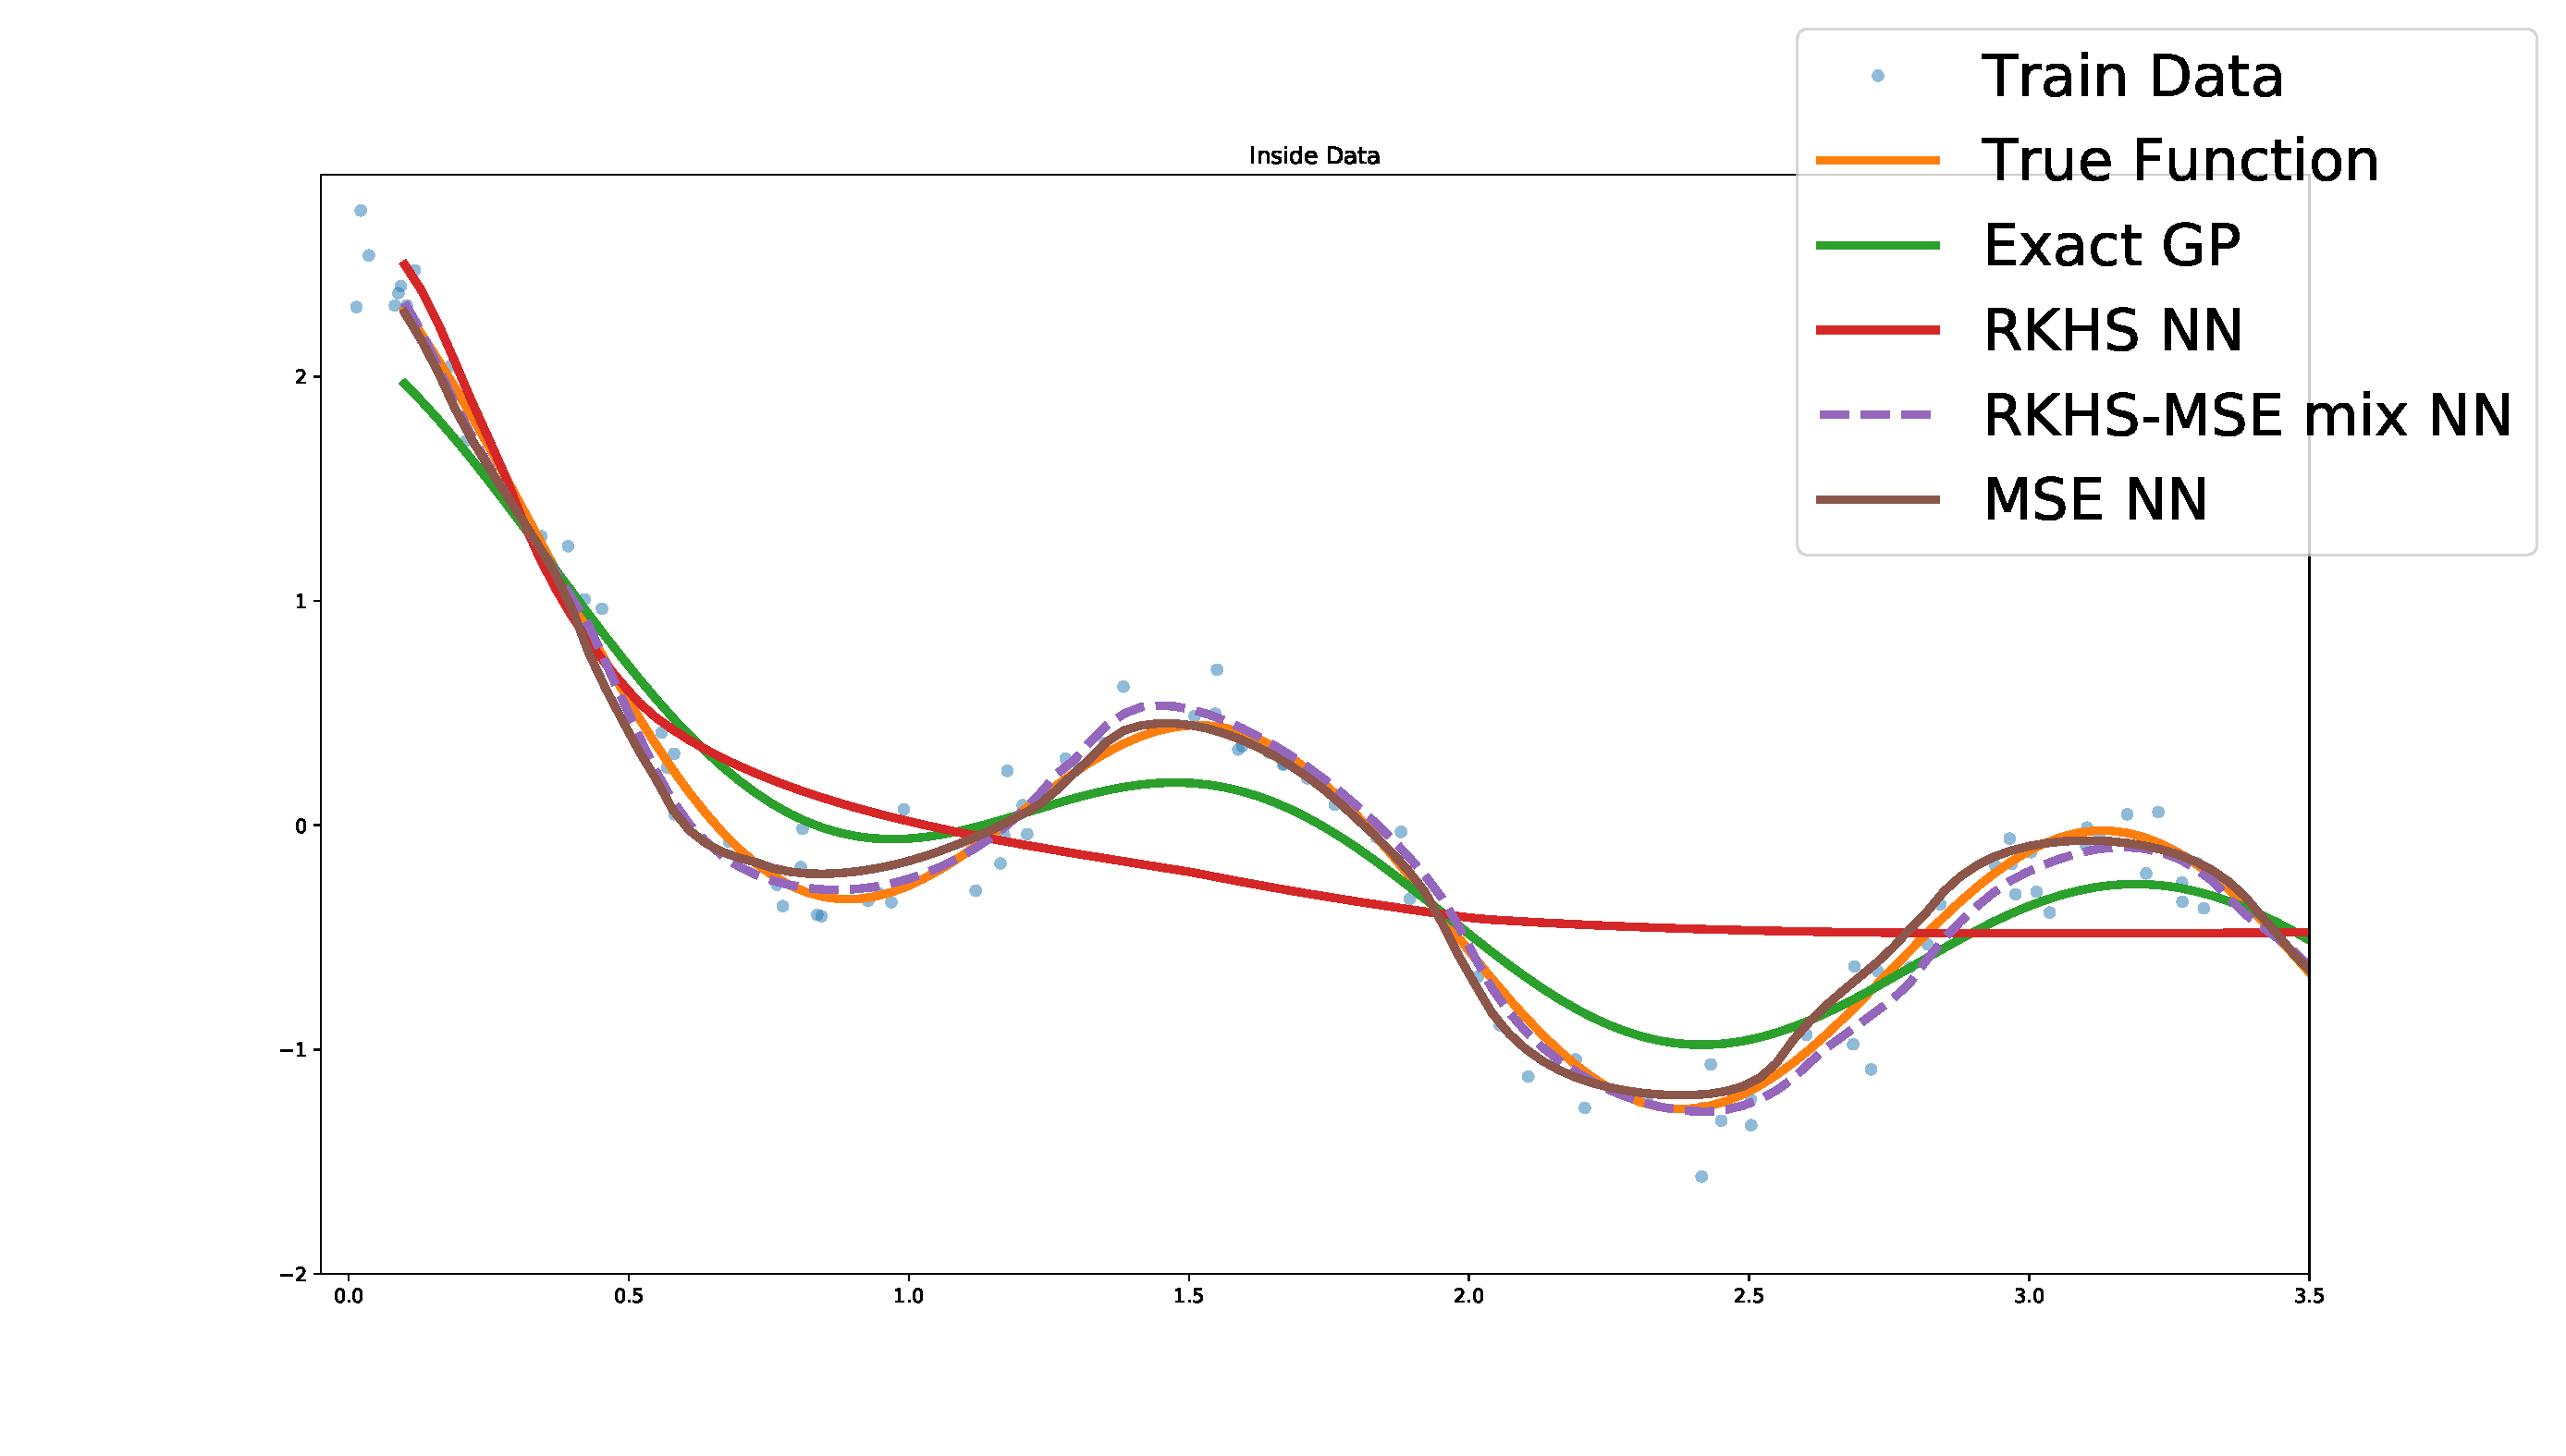
\includegraphics[scale=.35]{inside_data.pdf}



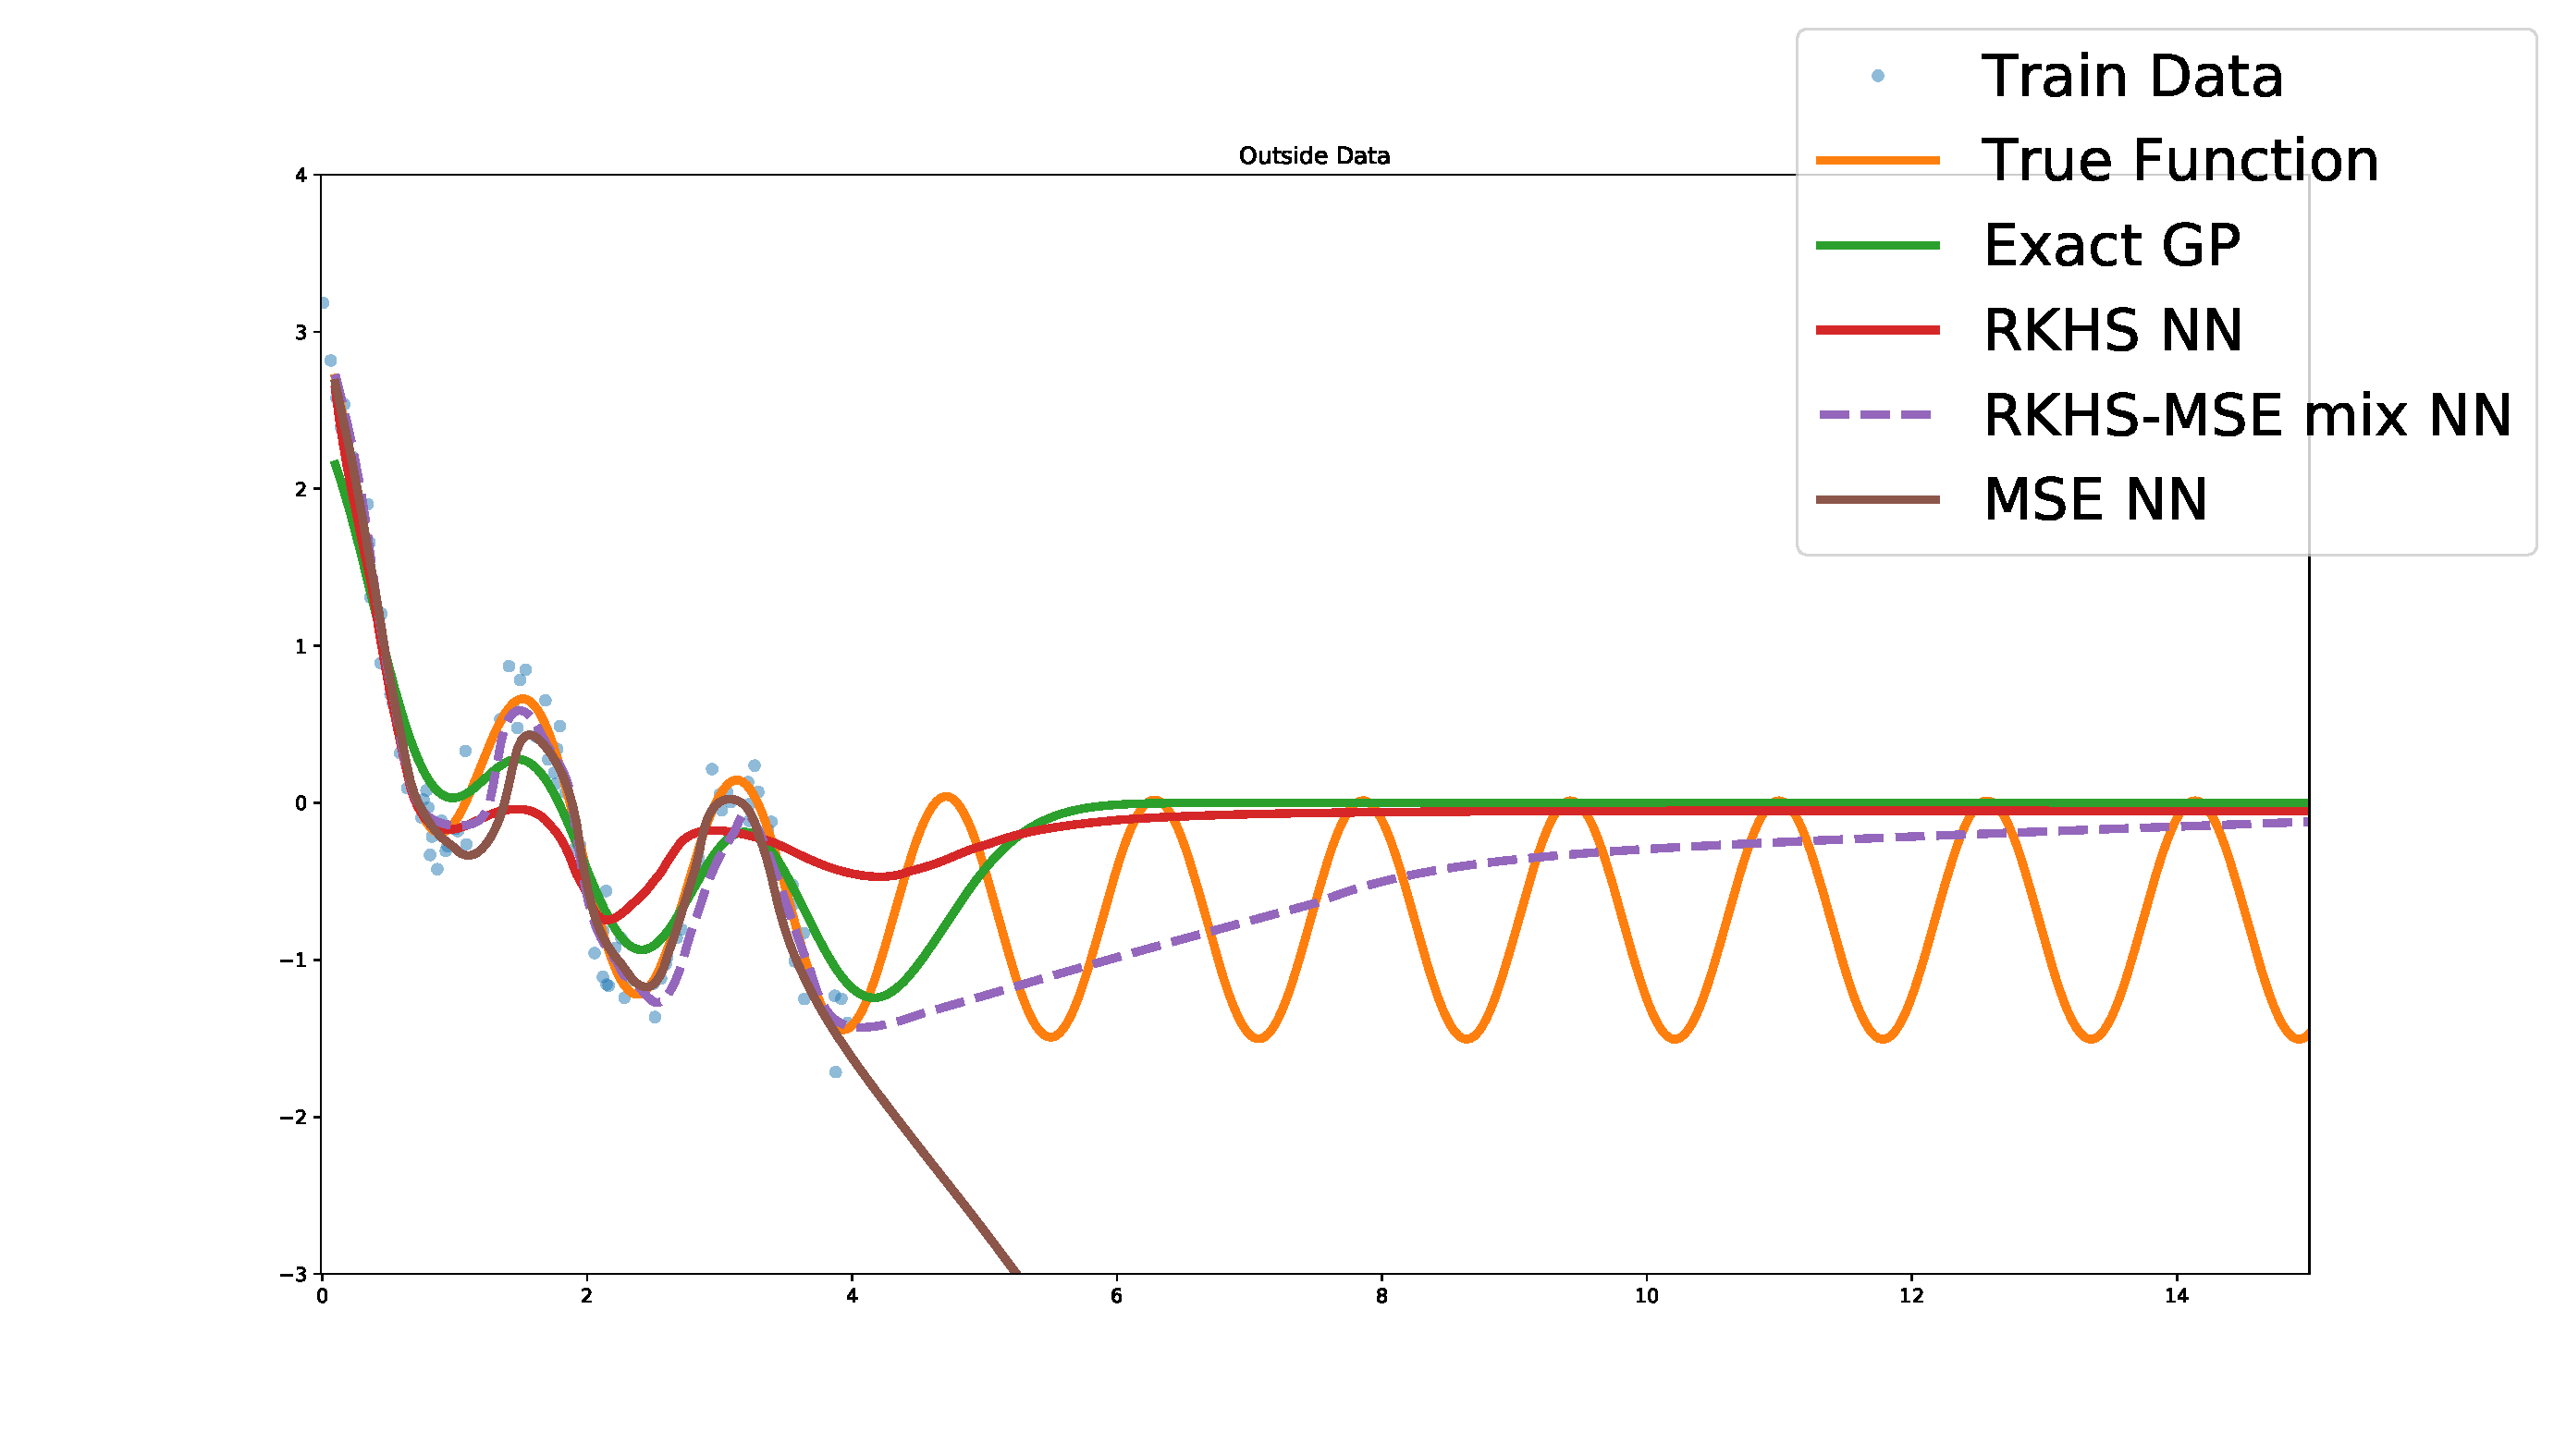
\includegraphics[scale=.35]{outside_data.pdf}

\begin{note}
There are a few observations to make. 
\begin{itemize}
\item The RKHS NN does not align well with the exact posterior mean inside the data, but it does revert back to the prior outside the training data like the posterior mean. Neither the RKHS NN nor the exact posterior mean fit the true data generating function well inside the training data.
\item The MSE NN fits the true data generating function well inside the training data, but it fits poorly outside the training data  
\item The RKHS-MSE mix NN fits the true data generating function well inside the training data and reverts back to the prior mean outside the training data.
\end{itemize}

So the neural network $g_{\theta}$ trained by the augmented loss function $l'_2(\theta)$ yields a better approximation to the true data generating function $f_0$ than the posterior mean inside the data and retains the nice property of reverting back to the prior mean outside of the data. Another thing to note is that once the network is trained, it is no longer necessary to store the training data and evaluation takes constant time with respect to the size of the training data unlike the posterior mean. So this approximation offers a computational improvement over the posterior mean as well.
\end{note}






\section*{References}



[1] \href{https://en.wikipedia.org/wiki/Reproducing_kernel_Hilbert_space}{Reproducing Kernel Hilbert Spaces, Wikipedia}

[2] \href{https://en.wikipedia.org/wiki/Representer_theorem}{Representer Theorem, Wikipedia}

[3] \href{https://github.com/carsonaj/Mathematics/blob/master/Introduction\%20to\%20Analysis/Introduction\%20to\%20Analysis.pdf}{Analysis Notes, My GitHub}

\end{document}
